\section{Test Regler}
Für den Test des entworfenen Reglers sind die Arbeitspunkte so gewählt, dass
diese im optimalen Arbeitsbereich der zwei Übertragungsfunktionen $G_5(s)$
und $G_7(s)$ liegen.
\begin{figure}[h!]
	\centering
	\begin{subfigure}{0.475\textwidth}
		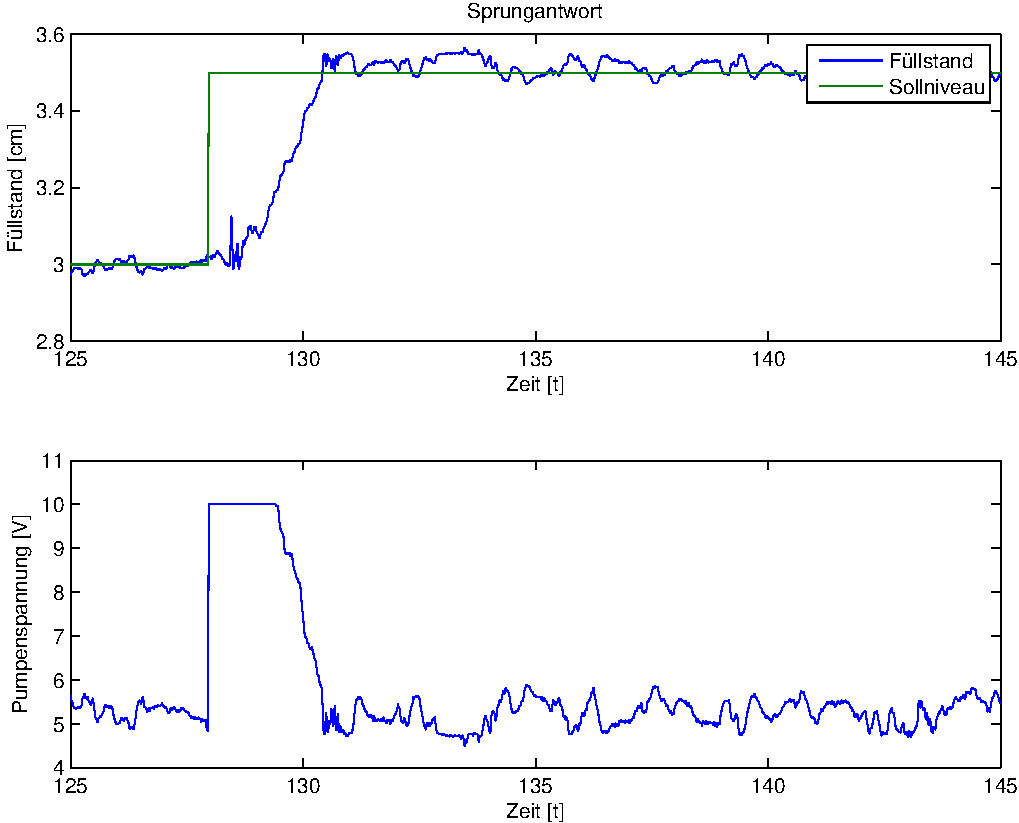
\includegraphics[width=1\textwidth]{12/step_g5.pdf}
		\caption{Sprungantwort im Arbeitsbereich von $G_5(s)$}
	\end{subfigure}
	\hfill{}
	\begin{subfigure}{0.475\textwidth}
		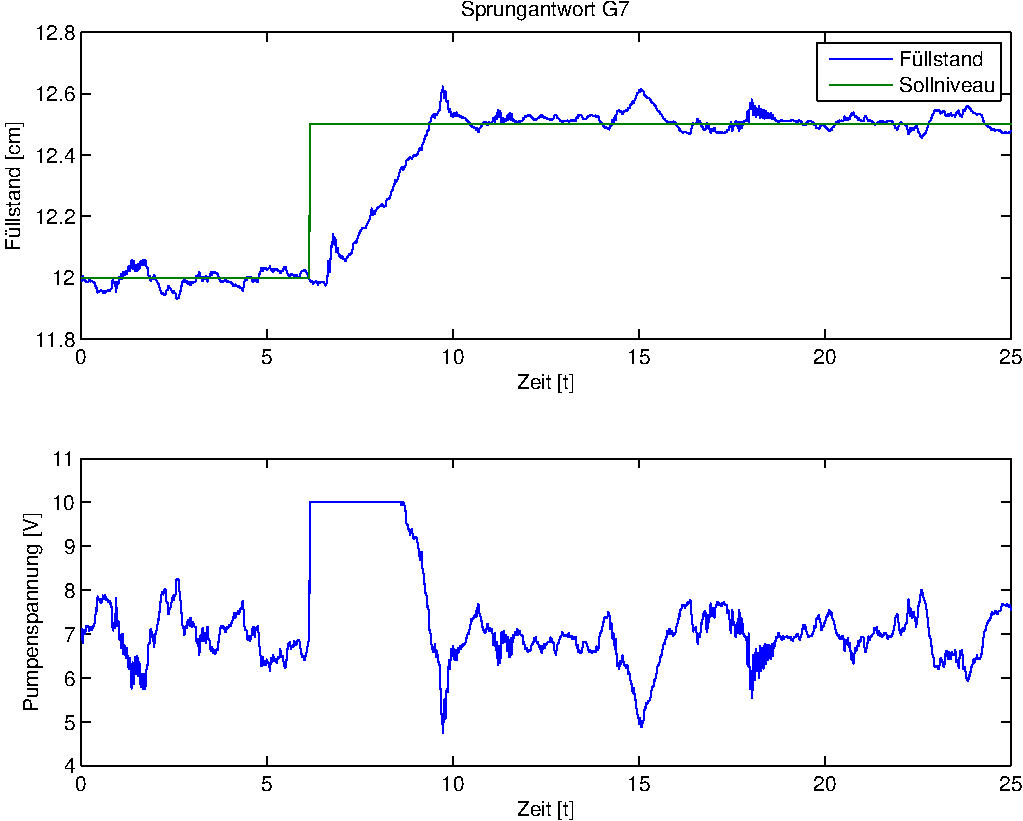
\includegraphics[width=1\textwidth]{12/step_g7.pdf}
		\caption{Sprungantwort im Arbeitsbereich von $G_7(s)$}
	\end{subfigure}
	\caption{Sprungantworten zu verschiedenen Arbeitspunkten}
\end{figure}
